\begin{surferPage}{쿠머의 $4$차식}
    1875년에 독일의 수학자 에두아르트 쿠머가 처음으로 $d$차 곡면의 최대 특이점의 개수 $\mu(d)$에 대해 질문을 던졌습니다. 
  
    그는 $\mu(4)=16$ 라는 것을 증명하였습니다. 그 이후 $16$개의 특이점을 갖는 $4$차식을 더 자세히 연구하였습니다. 이런 $4$차곡면 중 특히 아름다운 것들은 다음과 같은 식으로부터 만들어집니다.  
    \[\bigl(x^2+y^2+z^2-\mu^2\bigr)^2 - \lambda
    \,y_0\,y_1\,y_2\,y_3,\]
    여기서 $\mu$는 자유변수이고, $\lambda = \frac{3\mu^2-1}{3-\mu^2}$ 입니다; $y_i$ 는 정사면체의 각 면의 방정식으로 {\small
    $y_0=1-z-\sqrt{2}x$, \  
    $y_1=1-z+\sqrt{2}x$, \ 
    $y_2=1+z+\sqrt{2}y$, \ 
    $y_3=1+z-\sqrt{2}y$} 입니다. 이렇게 표현되는 모든 곡면들이 정확히 $16$개의 특이점을 갖는 것은 아닙니다. 하지만 대부분 $16$개를 가집니다. 
 

 \begin{center}
    \vspace*{-0.2cm}\hspace*{-0.2cm}
    \begin{tabular}{@{}c@{\,}c@{\,}c@{\,}c@{\,}c@{}}
      \begin{tabular}{@{}c@{}}
        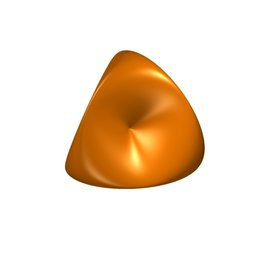
\includegraphics[height=1.4cm]{./../../common/images/kummer_0}
      \end{tabular}
      &
      \begin{tabular}{@{}c@{}}
        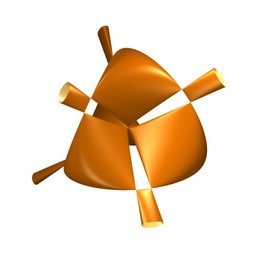
\includegraphics[height=1.4cm]{./../../common/images/kummer_1}
      \end{tabular}
      &
      \begin{tabular}{@{}c@{}}
        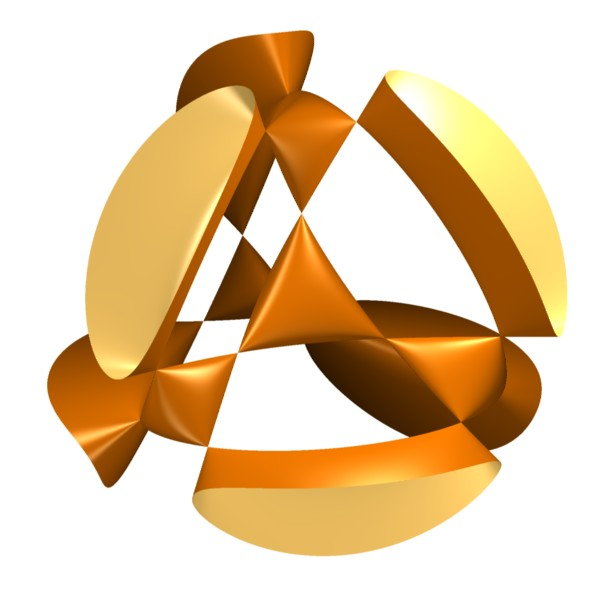
\includegraphics[height=1.4cm]{./../../common/images/kummer_2}
      \end{tabular}
      &
      \begin{tabular}{@{}c@{}}
        
\includegraphics[height=1.4cm]{./../../common/images/kummer_3}
      \end{tabular}
    \end{tabular}
  \end{center}
  \vspace{-0.2cm}  
   몇 개의 특이한 매개변수에 대해서는 일부 특이점들이 일치합니다.
\end{surferPage}
